\chapter{Аналитическая часть}

В данном разделе осуществляется анализ области исследования, включая описание концепции антикафе, классификацию доступных систем управления базами данных, формализацию поставленных задач и структуры данных, а также оценку имеющихся решений в этой области. На основе этого анализа формируется список пользователей, определяются сценарии использования в системе, и создаются схемы данных, включая диаграмму вариантов использования и диаграмму сущность-связь в нотации Чена.

Кроме того, основываясь на характеристиках данных, которые будут храниться в системе, выбирается наилучшая модель базы данных. В этой части работы также проводится анализ различных методов хранения данных, и выбирается наилучший метод для решения поставленной задачи.

\section{Анализ предметной области}

На протяжении всей свой жизни человек находится, развивается и живет в обществе, которое формирует ценности, стереотипы, и нормы поведения.
Но также в жизни человека важную роль играет организация его досуга, свободного времени, которое освобождено от других видов деятельности~\cite{anticafe-login}.

Антикафе --- заведение для реализации культурно-досуговой деятельности, в котором посетители обладают большой степенью свободы, чем кафе или рестораны, основной характеристикой которого является плата за проведенное время. 
Основная задача антикафе --- предоставить гостям рабочую, творческую или развлекательную атмосферу. 
Целью посещения таких мет является не утоления голода как такого, а приятное время провождение, развлечение и посещение тематических мероприятий и т.п.
Обычно антикафе состоят из одного большого зала или нескольких комнат, где люди свободно перемещаются и поэтому оно подразделяется на зоны:
\begin{itemize}
	\item <<Развитие>> --- пространство, где проводятся лекции, тренинги, курсы, интеллектуальные игры, мастер-классы и т.п.;
	\item <<Работа>> --- пространство, где можно спокойно поработать, т.е. представляет из себя коворкинг;
	\item <<Развлечение>> --- пространство под различные игры, концертов, кино и т.п.;
	\item <<Творчество>> --- пространство для реализаций творческой деятельности.
\end{itemize}

Также в одной из комнат есть зона с угощениями, в которой гости могут взять печенья или сладости, а также налить себе кофе, чай~\cite{anticafe-login}.

\section{Анализ существующих решений}

Формат заведения антикафе уже существует около десятка лет поэтому в данной области существуют информационная системы с механизмами бронирования для таких заведений, но у них есть недостатки. Наиболее популярными являются:
\begin{enumerate}
	\item Party Hard --- один из наиболее известных сайт антикафе, который предоставляет возможность просмотра информации о зонах и оформление брони без аккаунта~\cite{party-hard}; 
	\item Bizone --- сайт сеть антикафе, который предоставляет возможность просмотра информации зон, меню и оформление брони по звонку в антикафе~\cite{bizone};
	\item SpeedRent --- сайт бронирования развлекательных заведений, который предоставляет возможность просмотра информации о зонах и оформление брони в указанную дату и время~\cite{speedren}.
\end{enumerate}

Критерии, выделенные для сравнения существующих решений:
\begin{enumerate}
	\item возможность иметь аккаунт;
	\item меню --- предоставления списка меню блюд пользователю;
	\item бронирование --- система оформление записи о закреплении зоны за клиентом на указанное время;
	\item рейтинг --- формирование оценки зоны по оставленным отзывам;
\end{enumerate}

\begin{table}[ht]
	\begin{center}
		\begin{threeparttable}
			\caption{\label{tb:d} Категории и сведения о данных}
			\begin{tabular}{|p{4cm}|p{4cm}|p{4cm}|c|}
				\hline
				\textbf{Критерий} & \textbf{Party Hard} & \textbf{Bizone} & \textbf{SpeedRent} \\ \hline
				Возможность иметь аккаунт & нет & нет & есть\\ \hline
				Меню & нет & есть & нет \\ \hline
				Бронирование  & бронировать можно, но не на указанное время, после оформления онлайн брони надо согласовывать время по звонку & бронирование по звонку & есть \\ \hline
				Рейтинг & нет & нет & есть \\ \hline
			\end{tabular}
		\end{threeparttable}
	\end{center}
\end{table}

Все вышеперечисленные существующие решения не предоставляют пользователю необходимый функционал для принятий решения выбора. В результате, данная работа отличается от существующих решений тем, что она удовлетворяет все установленные критерии.

\section{Формализация задачи}

Необходимо спроектировать базу данных для хранения информации о пользователях, зонах, пакетах, инвентаре, меню, отзывах и бронях залов. Требуется разработать приложение, предоставляющее интерфейс для просмотра, добавления, изменения и удаления информации, хранящейся в базе данных. Необходимо реализовать три вида ролей — гость, авторизованный пользователь и администратор.

В рамках поставленной цели необходимо спроектировать и реализовать базу данных, содержащую информацию о зонах, меню, пользователях антикафе и позволяющую изменить хранящейся в ней информации. Разработать механизм бронирования зон в антикафе.

\section{Формализация данных}
Основываясь на анализе предметной области, можно выделить следующие категории данных:
\begin{itemize}
	\item пользователь;
	\item зона;
	\item бронь;
	\item отзыв;
	\item инвентарь;
	\item пакет;
	\item блюдо.
\end{itemize}

Сведения о каждой категории данных содержится в таблице~\ref{tb:data}.

\begin{table}[ht]
	\begin{center}
		\begin{threeparttable}
			\caption{\label{tb:data} Категории и сведения о данных}
			\begin{tabular}{|c|p{10cm}|}
				\hline
				\textbf{Категория} & \textbf{Сведения} \\ \hline
				Пользователь & ФИО, дата рождения, пол, телефон, email, пароль, права доступа, адрес, \\ \hline
				Зона & Название, тип, размер в кв. м., рейтинг, ограничение на количество людей в зоне \\ \hline
				Бронь & Пользователь, зона, пакет, дата бронирования, время начала и конца брони, количество людей, статус, дата и время создания брони, оплачена ли бронь, итоговая цена \\ \hline
				Отзыв & Пользователь, зона, оценка, дата и время создания, комментарий  \\ \hline
				Инвентарь & Название, тип, дата выпуска, описание, списан ли инвентарь \\ \hline
				Пакет & Название, тип, время проведение, стоимость, описание \\ \hline
				Блюдо & Название, тип, цена, описание \\ \hline
			\end{tabular}
		\end{threeparttable}
	\end{center}
\end{table}

\clearpage

На рисунке~\ref{fig:er} приведена ER-диаграмма сущностей в нотации Чена.

\begin{figure}[h]
	\centering
	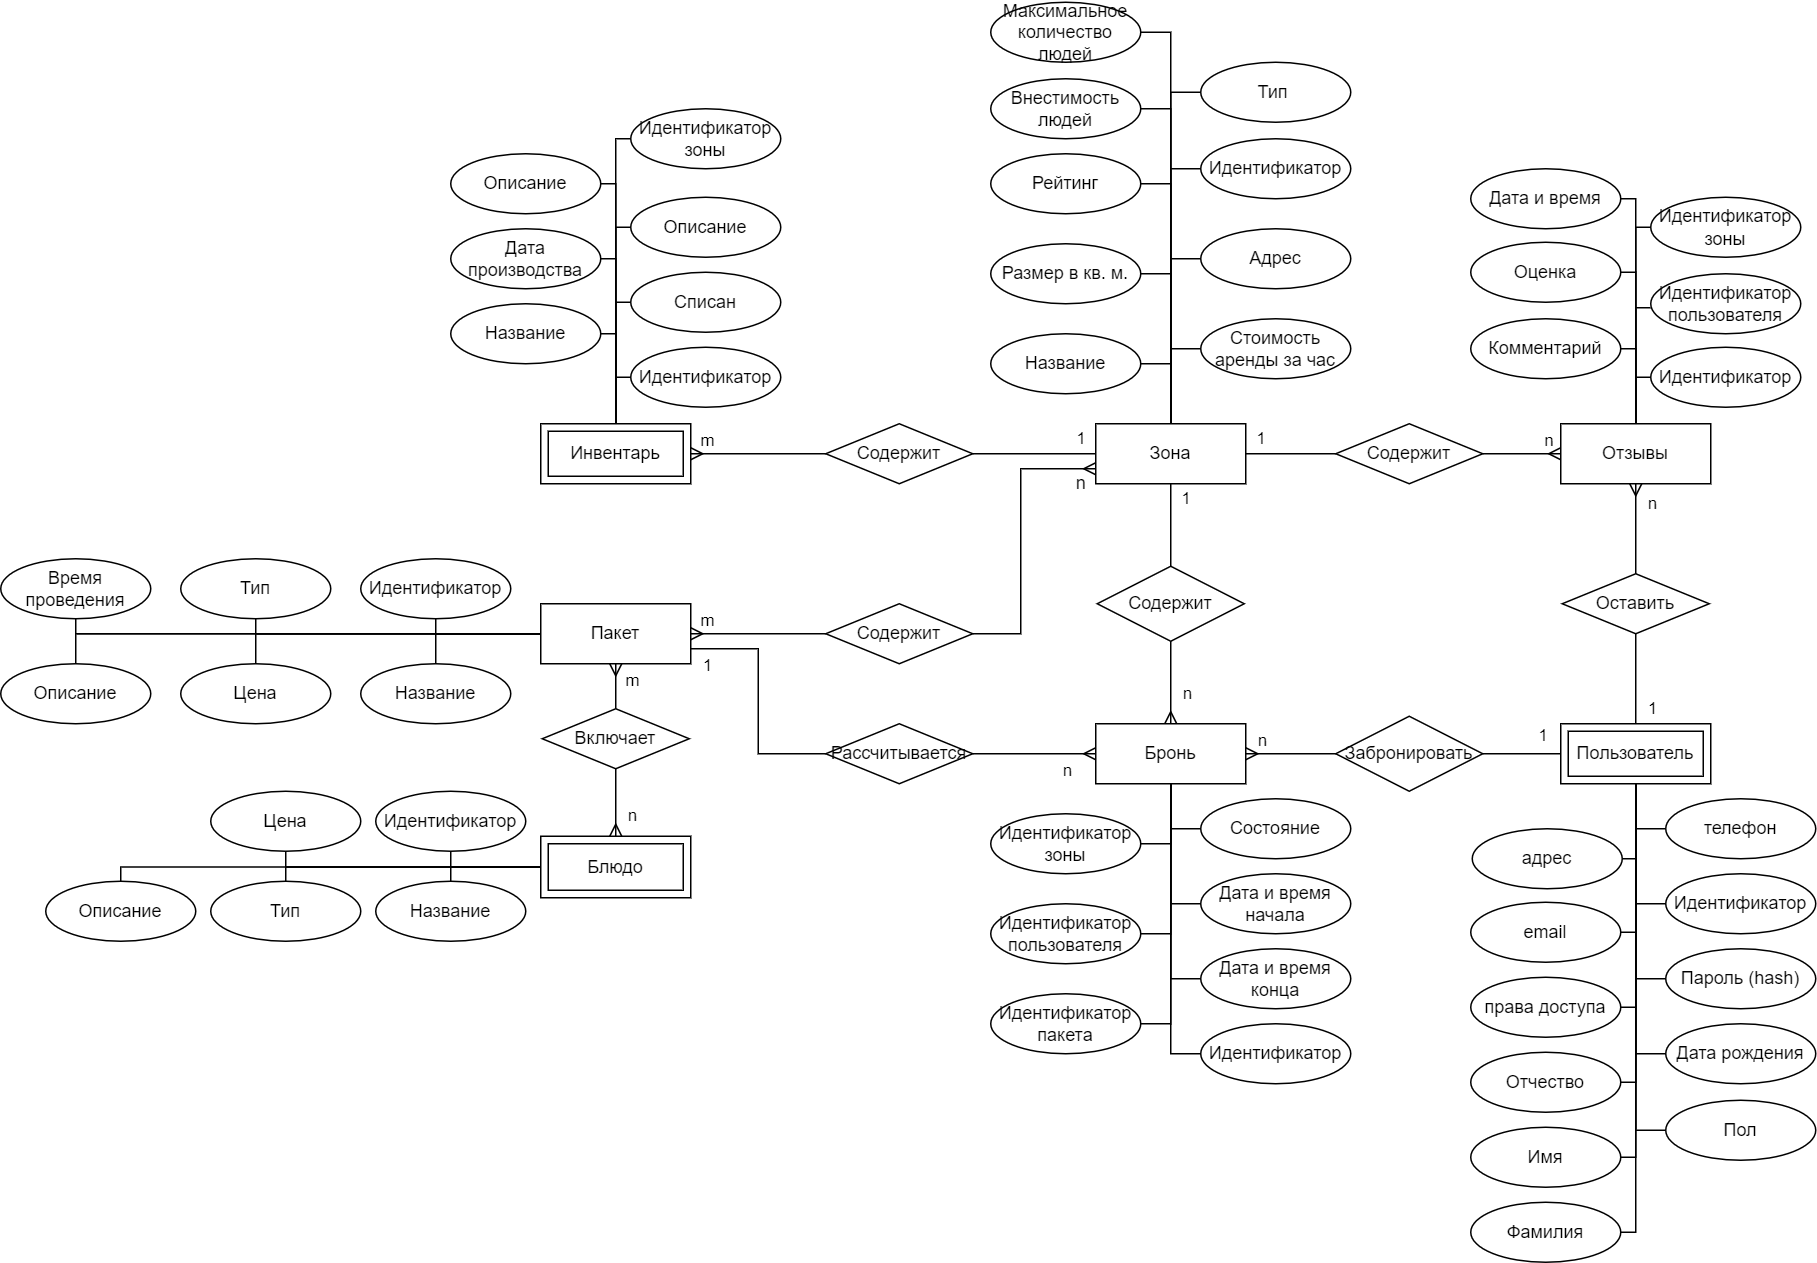
\includegraphics[width=0.9\textwidth]{img/er.png}
	\caption{ER-диаграмма сущностей}
	\label{fig:er}
\end{figure}

Для бронирования зоны антикафе пользователем необходимо разработать систему бронирования, которая основана на изменении статуса брони:
\begin{itemize}
	\item изначально авторизованный пользователь выбирает дату и время брони, после чего должна создаваться бронь с статусом <<временная бронь>>;
	\item после заполнения всех необходимых данных для брони пользователь подтверждает бронь и статус брони меняется с <<временной брони>> на <<забронировано>>;
	\item пользователь может отменить бронь, что приводит к изменению статуса брони на <<отменена>>;
	\item если бронь в статусе <<временная бронь>> и время для бронирования истекает, то такая бронь удаляется из базы данных;
	\item если бронь в статусе <<забронировано>>, то по истечению дата и времени конца брони она переводится в статус <<выполнена>>.
\end{itemize}

\clearpage

На рисунке~\ref{fig:status-booking} приведена диаграмма состояний брони зоны.

\begin{figure}[h]
 	\centering
 	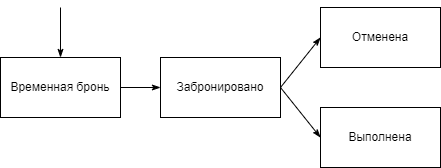
\includegraphics[width=0.55\textwidth]{img/status-booking.png}
 	\caption{Диаграмма состояний брони}
 	\label{fig:status-booking}
\end{figure}

\section{Формализация ролей}

Выделим группы пользователей разрабатываемой системы, исходя из предметной области поставленной задачи.

В системе выделяются 3 типа пользователей: 
\begin{itemize}
	\item гость --- неавторизованный пользователь, обладающий возможностями регистрироваться, входить в систему, просматривать данные зон, пакетов, блюд и отзывов;
	\item авторизованный пользователь обладает возможностью просматривать \\ данные зон, пакетов, блюд, отзывов, бронировать зону и отменять бронь зоны, оставлять и удалять отзыв, просматривать созданные брони;
	\item администратор --- авторизованный пользователь, обладающий возможностью просматривать, добавлять и менять данные зон, пакетов, инвентаря, блюд, отзывов, бронь и пользователей;
\end{itemize}

\clearpage

На рисунке~\ref{fig:use-case} приведена Use-case диаграмма. 

\begin{figure}[h]
	\centering
	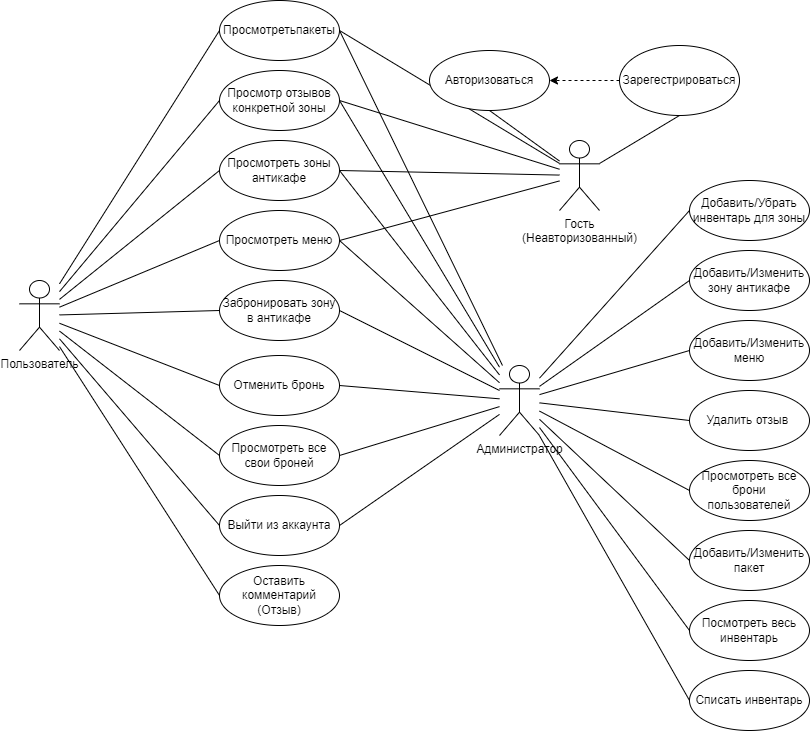
\includegraphics[width=0.8\textwidth]{img/use-case.png}
	\caption{Use-case диаграмма}
	\label{fig:use-case}
\end{figure}

\section{Анализ моделей баз данных}
База данных --- это некоторый набор перманентных (постоянно хранимых) данных, используемых прикладными программными системами какого-либо предприятия~\cite{intro-db-williams}.

По типу назначения базы данных делятся на:
\begin{enumerate}
	\item OLAP~\cite{intro-db-williams} --- это метод обработки данных, предназначенный для анализа больших объемов информации;
	\item OLTP~\cite{intro-db-williams} --- это метод обработки транзакций, предназначенный для выполнения операций в реальном времени.
\end{enumerate}

\clearpage

СУБД --- совокупность языковых и программных средств общего или специального назначения, обеспечивающих управление созданием и использованием баз данных~\cite{intro-db-williams}.

Основными функциями СУБД являются:
\begin{itemize}
	\item управление данными во внешней памяти;;
	\item управление буферами оперативной памяти;
	\item управление транзакциями;
	\item ведение журнала изменений в базе данных;
	\item обеспечение целостности и безопасности базы данных.
\end{itemize}

Модель данных --- это абстрактное и логическое определение объектов и его поведение, в совокупности составляющих доступ к данным, с которой взаимодействует пользователь~\cite{intro-db-williams}.
С помощью модели данных могут быть представлены объекты предметной области и взаимосвязи между ними.

СУБД различаются по модели данных, которая определяет архитектуру, структуры данных, обработку данных этой СУБД.
\begin{enumerate}
	\item Дореляционные модели. Наиболее известные представители:
	\begin{itemize}
		\item иерархические;
		\item сетевые;
		\item инвертированные списки. 
	\end{itemize}
	\item Реляционные модели данных.
	\item Постреляционные модели данных.
\end{enumerate}

\subsection*{Дореляционные базы данных}

Иерархическая БД состоит из упорядоченного набора деревьев; более точно, из упорядоченного набора нескольких экземпляров одного типа дерева~\cite{kuznecov-db}. 
В такой базе данных информация представлена в виде уровней, где каждый уровень имеет родительский и дочерний элемент. Эта модель данных особенно полезна для представления иерархических отношений и структур, как представлено на рисунке~\ref{fig:i-db}.

\clearpage

\begin{figure}[h]
	\centering
	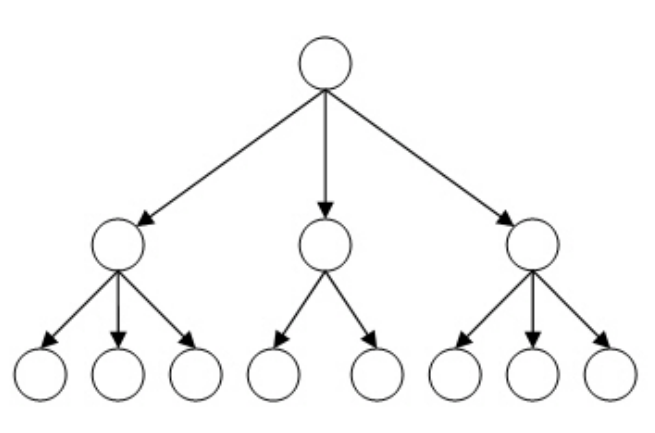
\includegraphics[height=0.2\textheight]{img/i-db.png}
	\caption{Структура иерархической модели данных}
	\label{fig:i-db}
\end{figure}

Сетевая модель данных --- логическая модель данных, являющаяся расширением иерархического подхода. 
В иерархических структурах запись--потомок должна иметь в точности одного предка, а в сетевой структуре данных потомок может иметь любое число предков~\cite{kuznecov-db}, как показано на рисунке~\ref{fig:network-db} 

\begin{figure}[h]
	\centering
	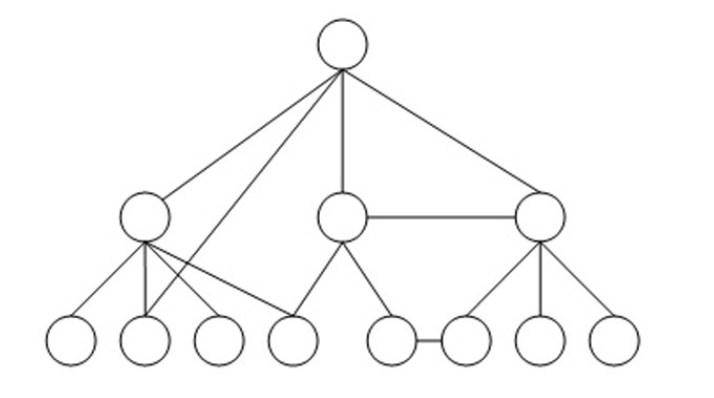
\includegraphics[height=0.2\textheight]{img/network-db.png}
	\caption{Структура сетевой модели данных}
	\label{fig:network-db}
\end{figure}

Дореляционные модели близки к управлению данными во внешней памяти на низком уровне, что при водит к наилучшему использованию памяти, но такие модели данных имеют сложность  использования, зависимость прикладных систем от физической организации. Так как логика процедуры выбора данных зависит от физической организации этих данных, то данная модель не является полностью независимой от приложения и как следствие приводит к усложнению действий изменений в базе данных, таких как добавление, удаление или изменение записей и связей.

\clearpage

\textbf{Реляционные базы данных}

Согласно Дейту реляционная модель состоит из трех частей, описывающих разные аспекты реляционного подхода.
 
В структурной части фиксируется, что единственной структурой данных используемой в БД, является n-арное нормализованное отношение и понятия структуры реляционной модели: тип данных, домен, атрибут отношения, схема отношения, схема БД, кортеж, отношение, первичный и потенциальный ключи~\cite{kuznecov-db}.

В целостной части реляционной модели определяются два требования целостности. 
Во-первых, требование целостности сущностей, которому соответствует кортеж отношений, то есть любой кортеж отношения обладает первичным ключом. Во-вторых, требование целостности по ссылкам, которое достигается соблюдением нормализованности отношений сложных сущностей представляемых в БД в виде нескольких отношений~\cite{kuznecov-db}.

В манипуляционной части модели утверждаются два механизма
манипулирования --- реляционная алгебра и реляционное исчисление.
Первый механизм базируется в основном на классической теории множеств, а второй --- на классическом логическом аппарате исчисления
предикатов первого порядка~\cite{kuznecov-db}. 

Основным достоинством использование реляционной модели заключается в простоте, понятности и удобстве физической реализации, что привело в широкому использованию, то есть формализация табличного представления данных, состоящего из записей и полей. Также независимость данных, то есть изменение структуры реляционной БД приводит к минимальным модификациям приложения. Важно отметить, что у реляционной модели отсутствие стандартные средства идентификации отдельных записей и сложность описания иерархических и сетевых связей.
Последние версии реляционных СУБД имеют некоторые
свойства объектно-ориентированных систем. 
Такие СУБД часто называют объектно-реляционным.

\textbf{Постреляционные базы данных}

Классическая реляционная модель предполагает неделимость данных, хранящихся в полях записей таблиц. Это означает, что информация в таблице представляется в первой нормальной форме. 
Существует ряд случаев, когда это ограничение мешает эффективной реализации приложений. 
Она использует трехмерные структуры, позволяя хранить в полях таблицы другие таблицы, расширяя таким образом возможности по описанию сложных объектов реального мира~\cite{postsql-db}. 

Постреляционная модель данных представляет собой расширенную реляционную модель, снимающую ограничение
неделимости данных, хранящихся в записях таблиц. 
Постреляционная модель данных допускает многозначные поля --- поля, значения которых состоят из подзначений. 
Набор значений многозначных полей считается самостоятельной таблицей, встроенной в основную таблицу~\cite{postsql-db}.

Достоинством постреляционной модели является возможность представления совокупности связанных реляционных таблиц одной постреляционной таблицей. Это обеспечивает высокую наглядность представления информации и повышение эффективности ее обработки.

\section*{Вывод}

В данном разделе была проанализирована предметная область, поставленная задача и рассмотрены способы ее реализации.
Так как задача предполагает использование разнообразных запросов различной сложности, приоритетным свойством модели данных является гибкость, простота использования и независимость от приложения, поэтому в качестве модели организации данных была выбрана реляционная модель БД.